\documentclass[{../../master}]{subfiles}
\graphicspath{{../..}}  % 個別コンパイル時の画像パスを解決する

\begin{document}

\section{URDFを記述する}

本節では,ROSにおいてロボットの構造をモデリングするためのフォーマットであるURDF(Unified Robot Description Format)と,URDFをプログラマブルに記述することのできるマクロパッケージであるXacro\footnote{\url{http://wiki.ros.org/xacro}}について解説します.

\subsection{URDFとは?}

URDFについての説明を引用します.\cite{what_is_urdf}

\begin{quote}
  URDF (Unified Robotics Description Format) は、製造業の組み立てライン用ロボット マニピュレーター アームや遊園地用のアニマトロニクス ロボットなどのマルチボディ システムをモデル化するために、学術界や産業界で使用される XML 仕様です。
\end{quote}

URDFでは,ロボットのモデルをリンク(Link)とジョイント(Joint)からなるツリー構造で表現します.
ボディやホイール,センサ等,駆動しないブロックをリンクとして扱い,リンクとリンクとの接続(固定,回転,直動,etc)をジョイントとして扱います.
URDFによってモデリングされたロボットは,最終的に図\ref{fig:urdf_tree}のような構造になります.

\begin{figure}[ht]
  \centering
  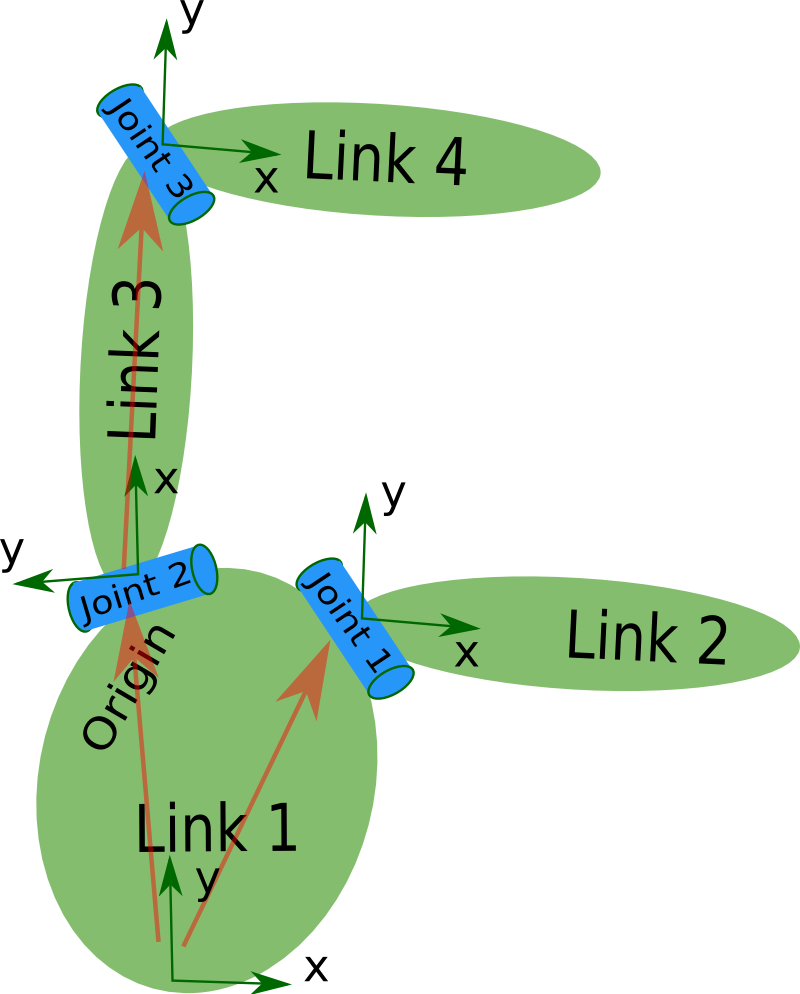
\includegraphics[width=70truemm, clip]{images/urdf_tree.png}
  \label{fig:urdf_tree}
  \caption{Tree Structure of URDF}
\end{figure}

URDFを記述することで,ロボットを構成する各リンクの位置関係やジョイントの属性を表すことができます.
また,URDFの各リンク/ジョイントに詳細なオプションを追加することで,シミュレーション用モデルを作成することもできます.

\subsection{何故URDFを書くのか?}

ROSの教本やチュートリアルでよく紹介されているURDFですが,実のところURDFを書かなくてもロボットの実機を動かすシステムを構築することができます.
URDFが提供するのは,ロボット座標系におけるセンサやアクチュエータ等の位置関係を示す座標変換であり,これはTFパッケージを用いることでも実現できるものです.
言い換えれば,TFを直接発行してロボットの各コンポーネントの座標変換を提供することができればURDFを記述する必要は無いという事です.

では,URDFを記述する理由はあるのでしょうか?
これはあくまで筆者の考えですが,以下のような利点があると考えます.

\begin{enumerate}
  \item ロボットの各コンポーネントの位置関係を一括で管理することができる
  \item ロボットの詳細な構造を可視化することができる
  \item 実機と同じモデルでシミュレーションを行うことができる
\end{enumerate}

URDFを記述することの大きな利点の1つとして,ロボットのモデルの可視化を行うことができるという点があると考えます.
リンクやジョイントの座標変換を提供するだけならTFパッケージを使うことで実現できるのですが,その場合モデルの可視化を行うことができません.
そのため,入力した数値が正しいのかどうかを検証するのが困難になります.
例えば,ロボットのハードウェアの設計を変更して,センサの位置が代わってしまったという場合を考えます.
TFパッケージとURDFのどちらを使う場合でも,新しいセンサの位置を3D CADの設計データから計算して数値を導出するのは同じですが,
TFパッケージを使う場合は可視化の手段が乏しいため,その数値が正しいかどうかを検証することが難しくなります.
一方でURDFを使う場合は,URDFファイルを編集\footnote{実際は\textsf{xacro}で記述した後にURDFをエクスポートすることが多いので,直接URDFファイルを編集することはありません.}し,
更新したモデルを\textsf{rviz}で可視化することで,センサの位置が正しい位置にいるのかどうかを目で確かめることができます.

また,副産物的な考え方ですが,実機用のURDFファイルにシミュレーションのためのオプションを追記することで,ロボットのシミュレーション環境を簡単に整えることが可能になります.
\textsf{ros\_control}\footnote{\url{http://wiki.ros.org/ros_control}}のフレームワークと合わせることで実機とシミュレーションで同一のコントローラを使ってロボットを動かすことができるため,SLAMやNavigation等のアプリケーションの開発を効率よく進められるようになります.

以上の理由から,ここではURDFを記述してロボットのモデリングを行うことを強く推奨します.
次の小節移行から,ADAMR2で実際に使用している\textsf{xacro}ファイルをもとに,URDFによるロボットの実践的なモデリングについて解説します.

\subsection{対向2輪ロボットの実機用URDFモデリング}

早速\textsf{xacro}を用いて実際に対向2輪ロボットの実機用URDFモデリングを行います.
\textsf{xacro}を用いるため,URDFを直接記述することはありませんが,URDFの記述に関する基礎知識が必要になります.
このセクションではURDF記述のチュートリアルについては取り扱わず,より実践的な内容を説明します.
URDFモデリングのチュートリアルはWeb上に大量に存在します.
この小節を読む前に,そちらを参照して基礎知識を身に付けてください.

これからモデリングする対向2輪ロボットの概要図を図\ref{fig:mobile_robot_structure}に示します.

\begin{figure}[ht]
  \centering
  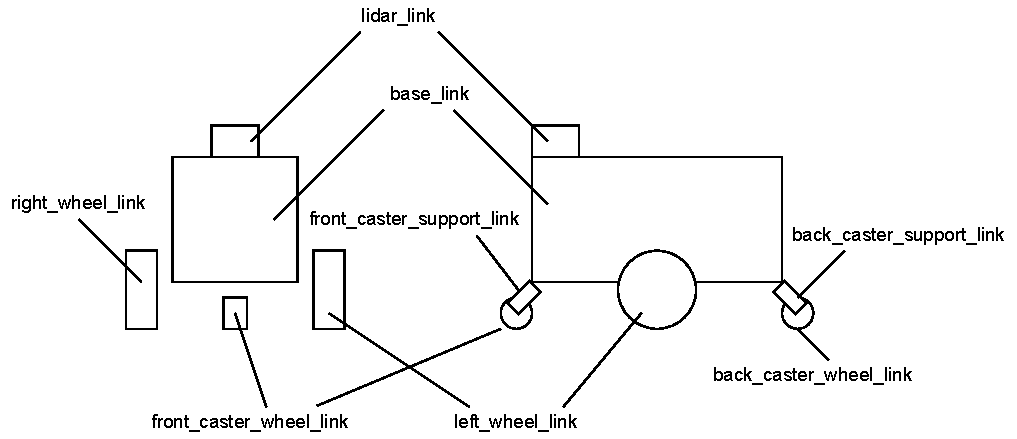
\includegraphics[width=100truemm, clip]{images/mobile_robot_structure.pdf}
  \caption{Link Structure of Diff-Drive Mobile Robot}
  \label{fig:mobile_robot_structure}
\end{figure}

\subsubsection{ディレクトリ構成}

慣習的に,ロボットのURDFモデルは\textsf{\*\_description}(\* はロボットもしくはプロジェクトの名前)という名前のROSパッケージに配置します.
ADAMR2プロジェクトならば「\textsf{adamr2\_description}」という名前になります.
URDFモデリングを始める前に,パッケージを作っておきましょう.
ビルド依存パッケージは無いので,パッケージ作成コマンドにオプションは必要ありません.

\begin{lstlisting}[language=sh, caption=Create a Package to put the URDF Model in]
catkin create pkg adamr2_description
\end{lstlisting}

\textsf{adamr2\_description}パッケージのディレクトリ構成はコード\ref{code:package_directory_structure}のようになります.

\begin{lstlisting}[language=sh, caption=Directory Structure of adamr2\_description, label=code:package_directory_structure]
adamr2_description/
  ├ launch/
  ├ meshes/
  ├ rviz/
  ├ urdf/
  ├ package.xml
  └ CMakeLists.txt
\end{lstlisting}

\textsf{launch/}ディレクトリには,URDFモデルの可視化を行うためのlaunchファイルを置きます.
\textsf{meshes/}ディレクトリには,STL形式のロボットの3Dモデルを置きます.
\textsf{rviz/}ディレクトリには,URDFモデル可視化時の\textsf{rviz}の設定ファイルを置きます.
そして,\textsf{urdf/}ディレクトリにxacroファイルを格納していきます.

\textsf{urdf/}ディレクトリの中身のディレクトリ構造はコードのようになります.

\begin{lstlisting}[language=sh, caption=Directory Structure of \textsf{urdf/}, label=code:urdf_directory_structure]
urdf/
  ├ base/
  │   └ base.xacro
  ├ caster/
  │   └ caster.xacro
  ├ lidar/
  │   └ lidar.xacro
  ├ wheel/
  │   ├ transmission.xacro
  │   └ wheel.xacro
  └ robot.xacro
\end{lstlisting}

\textsf{robot.xacro}がルートファイルです.
ルートファイルから各コンポーネントのxacroファイルをインクルードし,ロボットのモデルを作成します.
このファイルは最終的に\textsf{xacro}パッケージのノードを用いてURDFファイルに変換されます.

ロボットの主要コンポーネントである\textsf{base},\textsf{caster},\textsf{lidar},\textsf{wheel}のそれぞれに対してディレクトリを作り,その中に各々のxacroファイルを格納します.
\textsf{caster}及び\textsf{wheel}はロボットに2つずつ存在しますが,xacroファイルを複数作成する必要はありません.
共通のモジュールとしてxacroファイルを作成しておき,ルートファイルから読み込む際に名前や位置を付けることで各リンクを定義します.
また,\textsf{wheel}には\textsf{transmission.xacro}というファイルがありますが,これは\textsf{ros\_control}を用いたコントローラを作る際に必要となるオプションを設定するためのファイルです.


\end{document}